\documentclass[
	%a4paper, % Use A4 paper size
	letterpaper, % Use US letter paper size
]{jdf}

\addbibresource{references.bib}

\author{Nan Xiao}
\email{nanx@gatech.edu}
\title{CS6750 HCI Summer 2021:\\Assignment M1}

\begin{document}
%\lsstyle

\maketitle

\begin{abstract}
LinkedIn is one of the most popular social networks for professionals. Many of us rely on LinkedIn to expand connections and find new opportunities after graduation. In this project, we are going to study one task of LinkedIn - the searching function. First, we will define the problem space, such as what is searching function on LinkedIn and under what environment search function is used. Second, we will outline the user types for this study. Third, we will use 3 different needfinding methods to make a plan, which are  Items from the data inventory that will be connected to each needfinding plan. Also, the biases of each needfinding plan will be addressed.
\end{abstract}

\section{Problem Space}
The LinkedIn searching box sits in the top left corner for most of the pages as shown in Figure 1. The search function is an important starting point to create new connections for professionals. And the objective is to find a person using the searching function. There are many scenarios people are using this function. First, when people meet someone on professional occasions, they will use the exchanged name card to connect on LinkedIn. Or more conveniently, they can use the LinkedIn app to connect directly using QR code. Second, people meet in casual occasions normally will not change name card or add LinkedIn on the spot. But they generally know the names of each other. Later on, they may rely on the searching function to add these connections on LinkedIn. Third, people may want to connect to schoolmates after they graduate for a while. All they know maybe the names of their friends and they went to the same university. Fourth, people may want to connect to co-workers in the same company. The search criteria become name and company name in this case. There could be many more scenarios where people are using the searching function in LinkedIn. In this study, we will focus on finding the needs of one group of users, which will be elaborated on in the next section.
\begin{figure}[h]
	\centering
	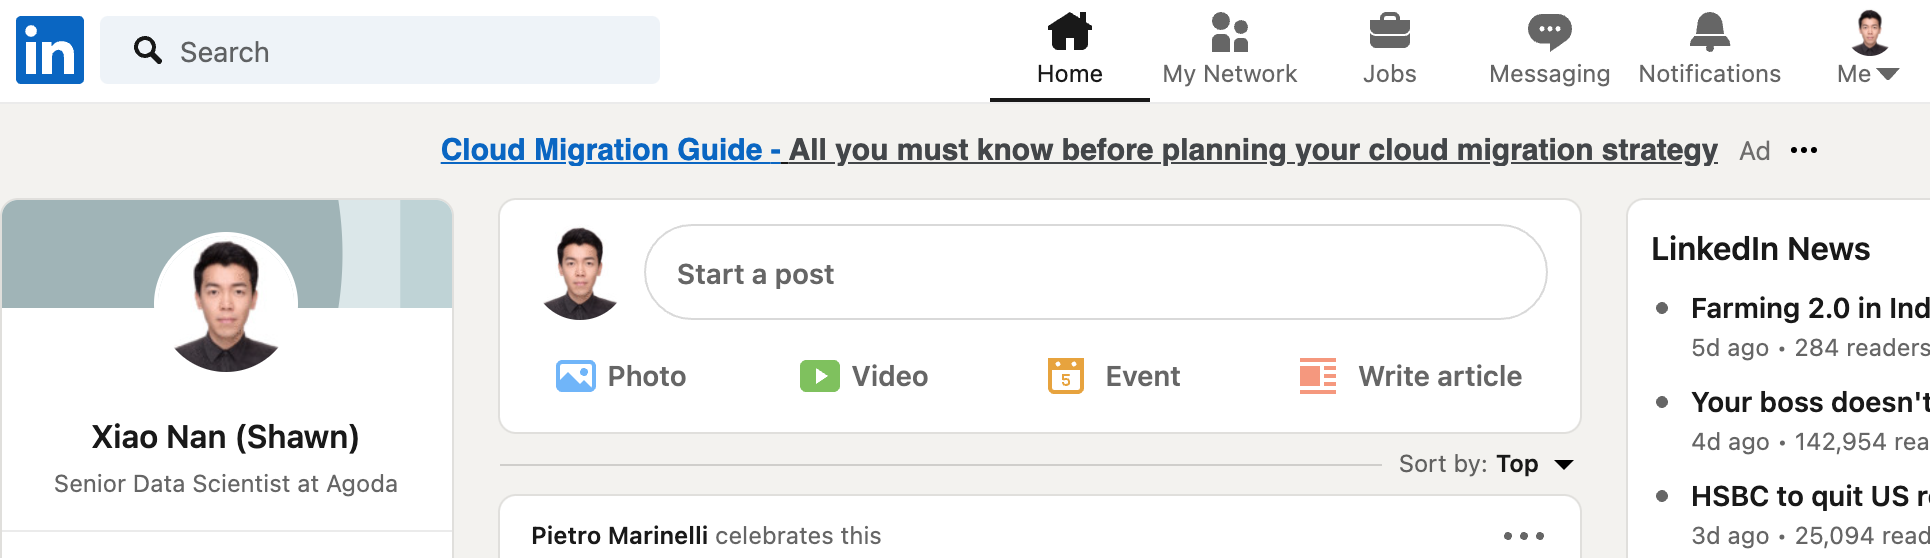
\includegraphics[height=6cm]{Figures/search_box.png}
	\caption{LinkedIn Search Box}
	\label{fig:search_box}
\end{figure}

\section{User Types}
The user types we are focusing on for this project are working adults in age group 25~34, which contains about 60\% of LinkedIn users (Statista, 2021). People belong to this age group are generally in the starting or early middle stage of their careers. Expanding professional network is also an important task for these group of users. Within this age group, the design will cater for both expert and novice users of LinkedIn, people with 1-3 years of working experiences and those with 4-10 years of working experiences, people with financial occupations and people working in IT industry. It will be summarized in below table:

\begin{table}[h] % [h] forces the table to be output where it is defined in the code (it suppresses floating)
	\caption{User Types for LinkedIn Search Function}
	\small % Reduce font size
	\centering % Centre the table
	\begin{tabular}{L{0.27\linewidth} L{0.17\linewidth} L{0.17\linewidth} L{0.17\linewidth}}
		\textbf{User Type} & \textbf{User Level of LinkedIn} & \textbf{Working Experience} & \textbf{Occupation} \\
		\toprule[0.5pt]
		Fresh software engineer & Novice & 1-3 yrs & IT\\
		\midrule
		Seasoned trader & Expert & 4-10 yrs & Financial\\
		\midrule
		Senior developer & Expert & 4-10 yrs & IT\\

	\end{tabular}
\end{table}

The motivations can vary for different user types. Fresh graduate with few connections may be interested more in connect to school-time classmates. While seasoned professionals may want to expand the connection in a specific area. People in the IT industry may want to connect to the same industry to see if there are any new opportunities. The task is similar but the motivations, the audience and the needs are very different. (Joyner, 2021) We will use needfinding methods in the next session to find the needs for all user types. 

\section{Needfinding Plan 1 - Participant observation}
\subsection{Needfinding Method - Participant observation}
The first needfinding method is Participant observation. In participant observation, the research will be working as a participant observer and observe what are the needs to accomplish the task. In this case, I will be the participant for this exercise and observe different needs to accomplish the task of finding a person on LinkedIn in a different environment. 

First, on the different page, I may need to use the searching function differently. But currently, in the LinkedIn only \emph{Jobs} page has a different design (as in figure 2). I probably would expect the search function to search my contact in \emph{My Network} page and chat history in \emph{Messaging} page. In the experiment, I will try to search on each page and see if the search result matches my intention.

\begin{figure}[h]
	\centering
	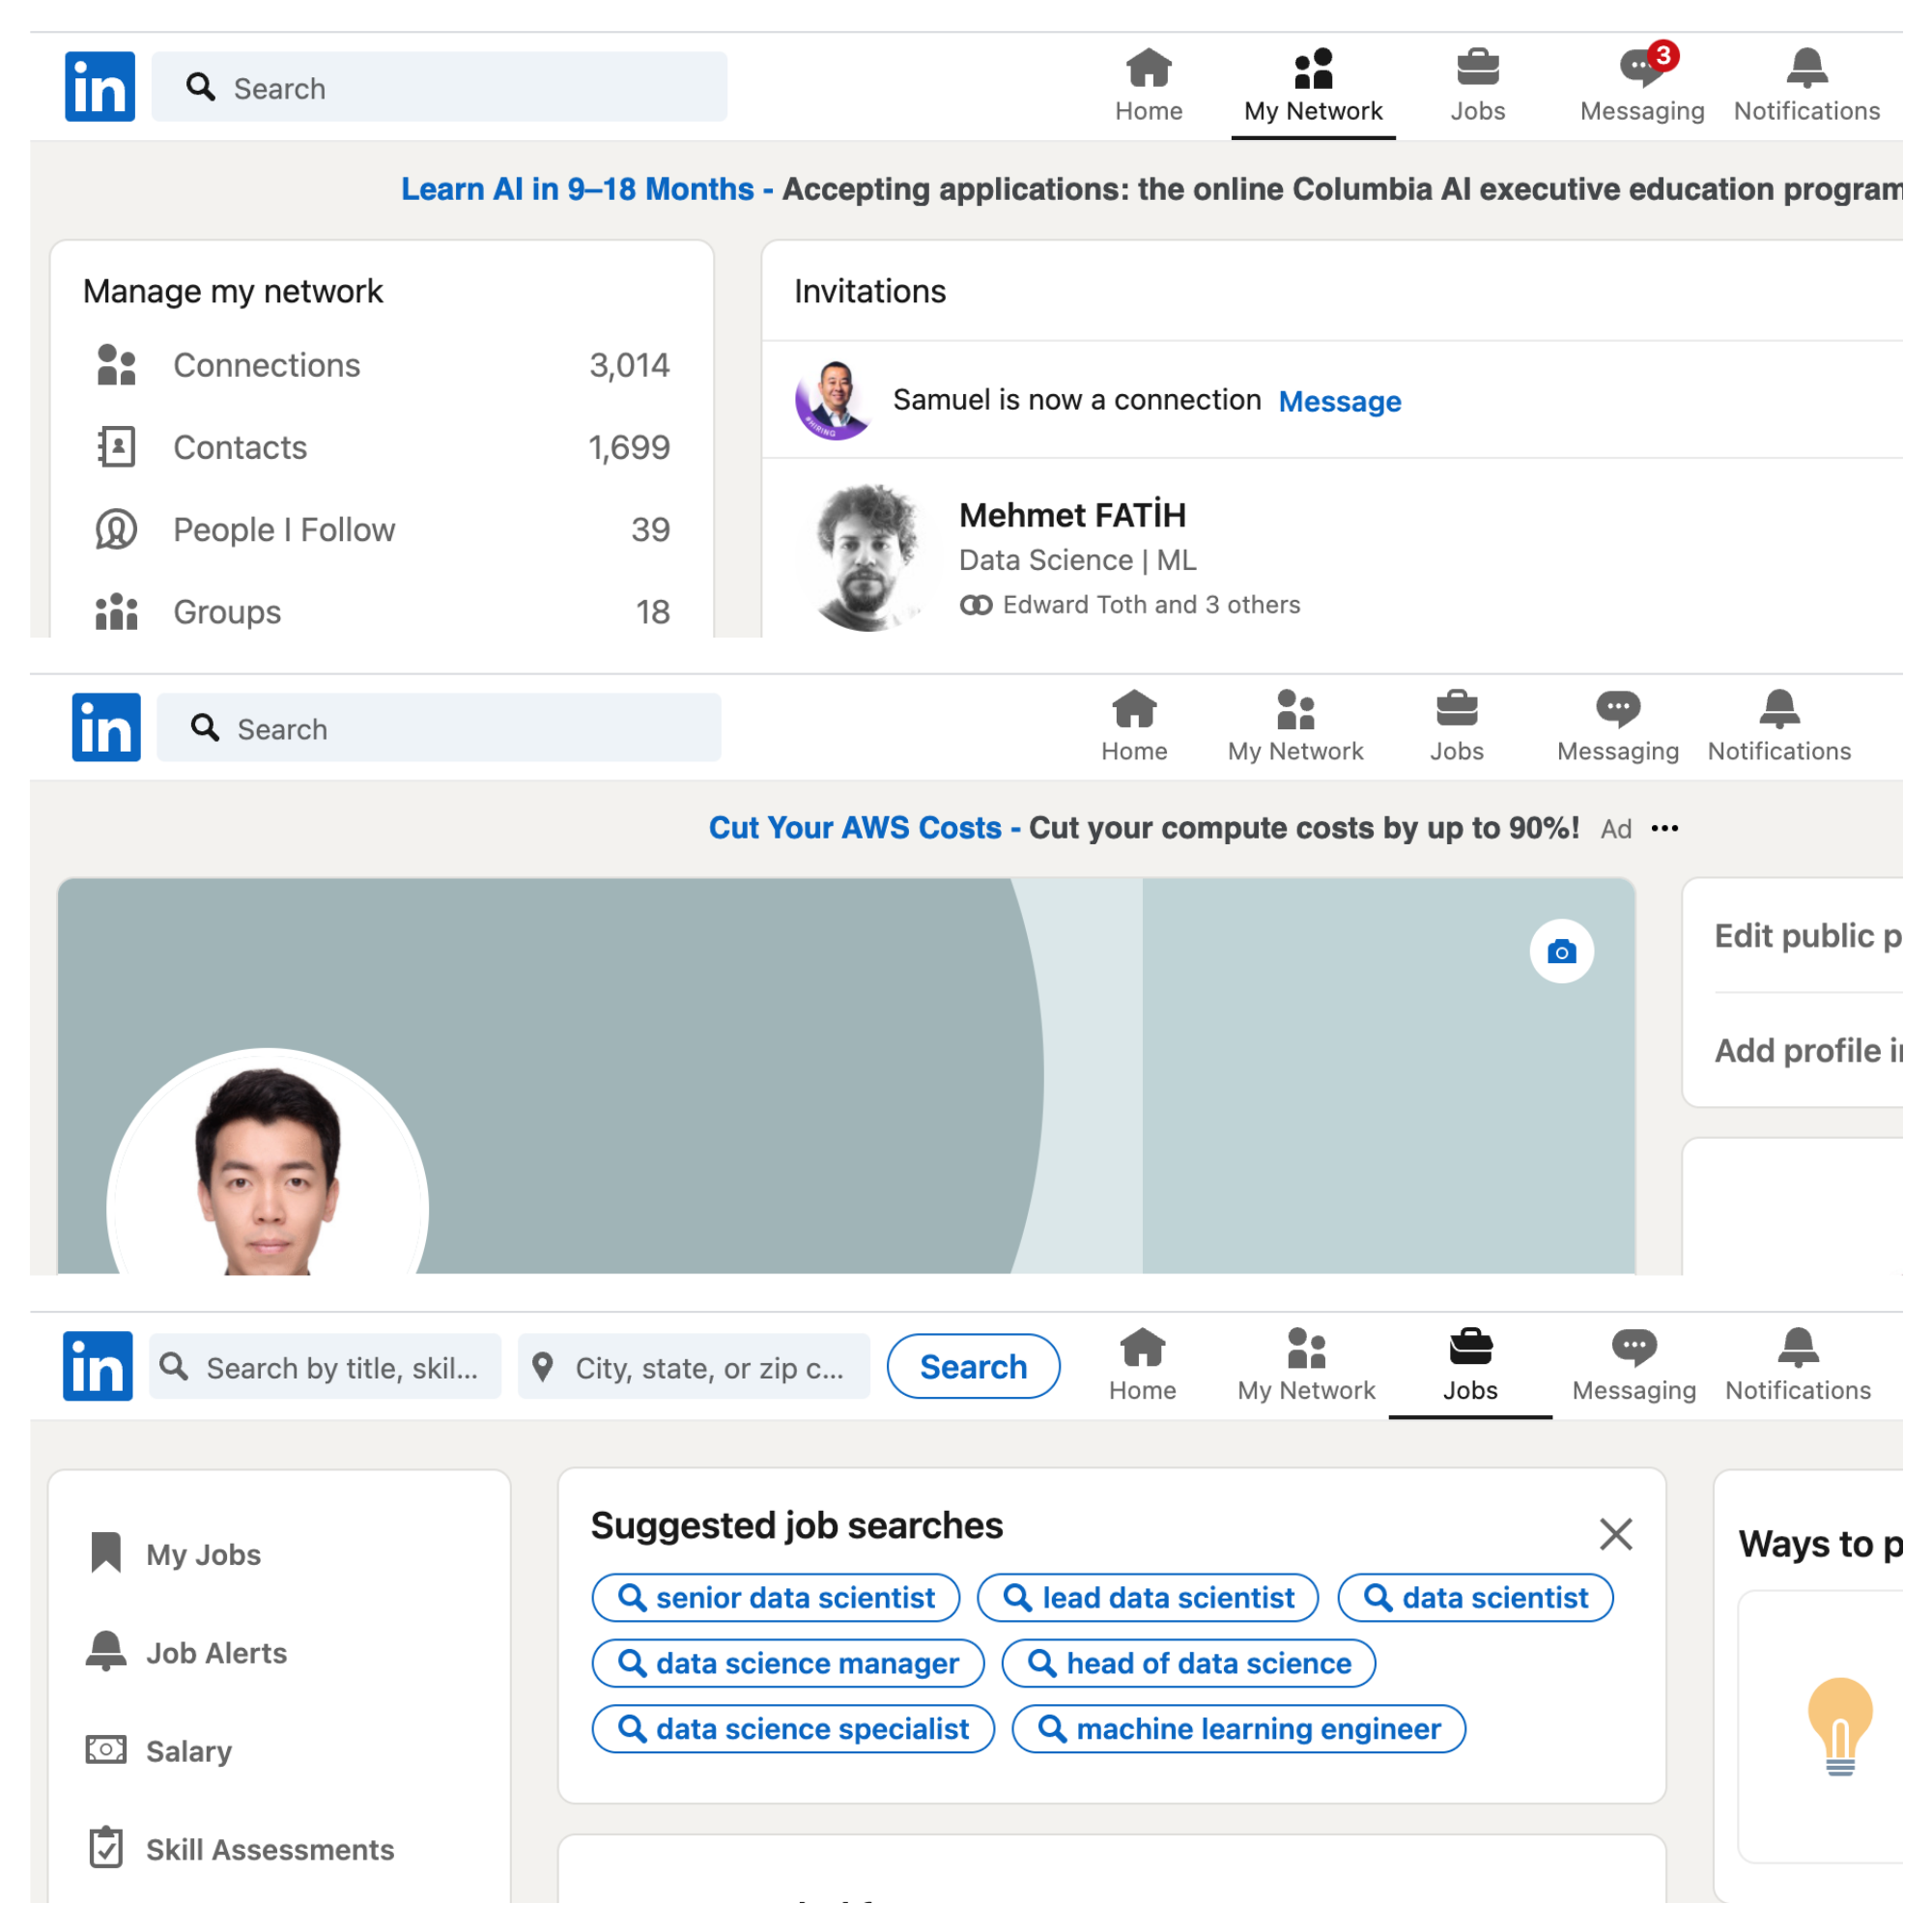
\includegraphics[height=10cm]{Figures/search_box2.png}
	\caption{LinkedIn Search Boxes are the same except in Jobs page}
	\label{fig:search_box2}
\end{figure}

Second, when I'm attending a conference, I may want to add people through mobile app searching. It might make sense for the app to be able to scan name card. Due to COVID-19, this environment is not easily testable. But we do have a worldwide town hall and tech summit that I may want to connect to the speakers. I will go through that process to understand whether the LinkedIn search function is good at searching people from video conference context.

\subsection{Data Inventory - Participant observation}
Below table summarized data inventories in this participant observation.

\begin{table}[h] % [h] forces the table to be output where it is defined in the code (it suppresses floating)
	\caption{Data Inventory - Participant observation}
	\small % Reduce font size
	\centering % Centre the table
	\begin{tabular}{L{0.1\linewidth} L{0.1\linewidth} L{0.1\linewidth} L{0.1\linewidth} L{0.1\linewidth} L{0.1\linewidth} L{0.1\linewidth}}
		\textbf{Who} & \textbf{Where} & \textbf{Context} & \textbf{Goal} & \textbf{Need} & \textbf{Tasks} & \textbf{Subtasks}\\
		\toprule[0.5pt]
		Me & Desktop & My Network & Find co-worker & Connect with colleague & Find and Connect to colleague & Search by name, filter by company, send invitation\\
		\midrule
		Me & Mobile & Homepage & Find speaker & Connect with speaker & Find and Connect to speaker & Search by full name, send invitation\\

	\end{tabular}
\end{table}


\subsection{Biases - Participant observation}
Participant observation can help in qualitative research, getting insights, contextual data and preparing interview and survey questions. It is an important needfinding method to start with. However, remember "You are not your user!".(Joyner, 2021) Participant observation can be biased if you overly represent your own experience. (Joyner, 2021) I may get confirmation biases in the participant observation, and ignore the useful data that does not match my presumption. It is useful to check the insights from participant observation in Interview and Survey to eliminate confirmation biases. Also, I may get Observer biases that I tend to see what I want to see and ignore other facts. Interviews and Surveys are also helpful to reduce the Observer biases.

\section{Needfinding Plan 2 - Interviews}
\subsection{Needfinding Method - Interviews}
The second needfinding method is Interviews. In this experiment, interview questions will be from the previous participant observation. Through the previous method, I will have some hypothesis from my participation experience. But they could be biased. For example, when I search a person's name "Oliver", and would like to apply company name as a filter. On the search result page, if I click the Company button, it will bring me to the result page of companies named "Oliver" instead of using a company name as a filter for people searching results. From the participant observation, I find a need to fix the misleading "Company" button. However, that might not be the same case for other people and it could be a biased need. I will collect interview questions based on my participant observations and ask the user types as defined in section 2.

To make interviews more effective, we need to make sure below 5 points (Joyner, 2021):
\begin{enumerate}
	\item Focus on Who, When, What, Where, Why, How, ask open-ended questions.
	\item Be aware of bias, phase questions in a neutral way.
	\item Listen, make sure participant do the most of talking.
	\item Organize the interview.
	\item Practice the questions on friends or families first.
\end{enumerate}

\begin{figure}[h]
	\centering
	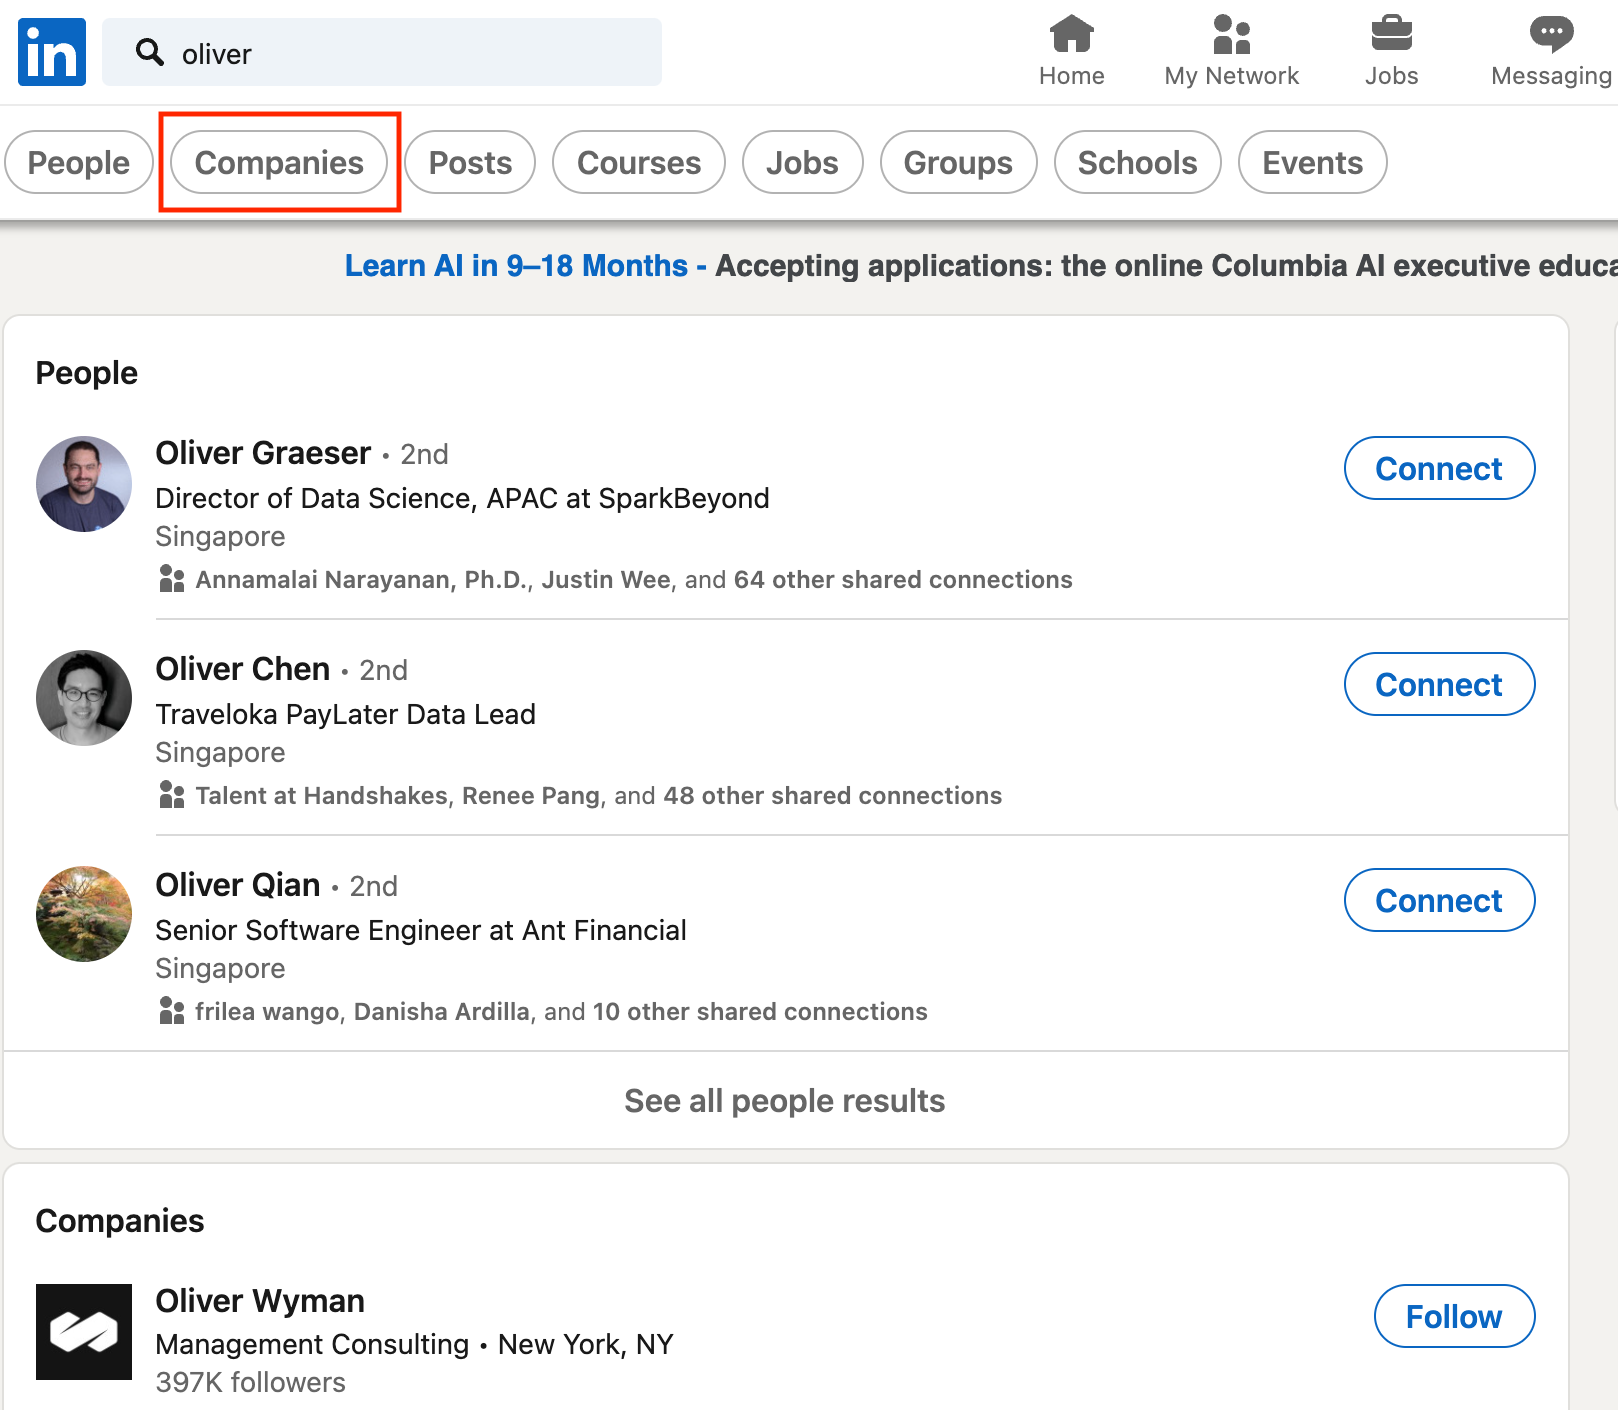
\includegraphics[height=10cm]{Figures/search_people.png}
	\caption{The "Companies" button is not a filter, but showing company results}
	\label{fig:search_people}
\end{figure}

\subsection{Data Inventory - Interviews}
Below table summarized data inventories in the Interviews method.

\begin{table}[h] % [h] forces the table to be output where it is defined in the code (it suppresses floating)
	\caption{Data Inventory - Interviews}
	\small % Reduce font size
	\centering % Centre the table
	\begin{tabular}{L{0.1\linewidth} L{0.1\linewidth} L{0.1\linewidth} L{0.1\linewidth} L{0.2\linewidth} L{0.2\linewidth}}
		\textbf{Who} & \textbf{Where} & \textbf{Context} & \textbf{Goal} & \textbf{Need} & \textbf{Tasks}\\
		\toprule[0.5pt]
		Senior Developer & Desktop Homepage & Teammate leaving company & Connect with colleague & Search function can easily identify teammate's profile & Search by name, find profile and evaluate\\
		\midrule
		Junior PM & Desktop Homepage & New-joiner in the company & Find new-joiner's background & Search function can easily identify new-joiner's profile & Search by name, find profile and evaluate \\
	\end{tabular}
\end{table}

We can collect the data of interviewee's feedback about how easy they can accomplish their goal, what are their needs to improve the interface, and also whether the needs from participant observation valid to them. Through this interview process, we can have more insights into the interface.

\subsection{Biases - Interviews}
If the questions are not open-ended or have a certain tendency, that would introduce biases that the response is bounded by our questions. Also, we need to be aware of social desirability bias. So we need to frame the questions as neutral as possible, and open-ended. Finally, we need to avoid recall bias by asking the participants as soon as possible after they finish the task. Otherwise, the participants may forget the details of the experiments.

\section{Needfinding Plan 3 - Surveys}
\subsection{Needfinding Method - Surveys}
The third needfinding method is Surveys. When we have enough insights about the tasks and needs under different context using qualitative research, we can have more data support by using quantitative research method like surveys. The first two needfinging methods can easily be biased as discussed above. Surveys can help to reduce those biases. Needs from the previous 2 needfinding methods will be rephrased so that the participant can respond in a quantifiable number. For example, a need from participant observation - the confusing button of "Companies" in the search result page should be replaced by filters. In the surveys, a question can be phrased as "On a scale 1 - 5, 1 being the easiest, how much effort for you to find company filter in the people search result"

To make surveys more effective, we need to make sure below 5 points (Joyner, 2021):
\begin{enumerate}
	\item Less is more. Ask minimum questions necessary.
	\item Be aware of bias, phase questions in a neutral way.
	\item Tie them to the inventory.
	\item Test it out. Have co-workers test survey questions before sending them out.
	\item Iterate and revise surveys according to the tests.
\end{enumerate}

\subsection{Data Inventory - Surveys}
Below table summarized data inventories in Surveys method.
\begin{table}[h] % [h] forces the table to be output where it is defined in the code (it suppresses floating)
	\caption{Data Inventory - Surveys}
	\small % Reduce font size
	\centering % Centre the table
	\begin{tabular}{L{0.15\linewidth} L{0.15\linewidth} L{0.15\linewidth} L{0.1\linewidth} L{0.1\linewidth} L{0.2\linewidth}}
		\textbf{Who} & \textbf{Where} & \textbf{Context} & \textbf{Goal} & \textbf{Need} & \textbf{Tasks}\\
		\toprule[0.5pt]
		Group of Senior Developers & Desktop Homepage & Recall when you were searching someone on LinkedIn & Successfully found & Change of interface & Search by name, find profile and evaluate\\
		\midrule
		Group of Junior Analysts & Desktop Homepage & Recall when you were searching someone on LinkedIn & Successfully found & Change of interface & Search by name, find profile and evaluate \\
	\end{tabular}
\end{table}

We can collect quantitative data from surveys that give us a more unbiased view of needs. For each need, we will have a question for that and a series of data points we can calculate the score for that need. For example, if after the survey the need to remove "Companies" button is -5, then
it suggests that need is biased to myself and generally it is not a real need for the users.

\subsection{Biases}
Surveys are good for gather lots of users' data. But it can also introduce several biases. We must neutrally phase the survey question or the response may suffer biases. Also, the participants need to be selected randomly to avoid Voluntary response bias. The survey is likely to have recall bias since it does not occur within the task context. And finally, we must allow anonymous responses or the survey may suffer from social desirability bias as well. It's best to combine the 3 needfinding methods and iteratively improve the needfinding.

\section{Needfinding Plan Conclusion}
From the above analysis, we can see that, it's better to combine several needfinding methods to have more in-depth but less biased needs for our selected user types and problem spaces. Both qualitative research and quantitative research are important methods for us to find the needs of our users.

\section{References}
[1] Statista. (2021, February 9). Distribution of LinkedIn users worldwide as of January 2021, by age group. https://www.statista.com/statistics/273505/global-linkedin-age-group/

[2] Joyner, D. (2021). User Types. Udacity.

https://classroom.udacity.com/courses/ud400/lessons/9662642568/

concepts/96759245490923

[3] Joyner, D. (2021). 5 Tips: Interviews. Udacity.

https://classroom.udacity.com/courses/ud400/lessons/9662642568/

concepts/97510951660923

[4] Joyner, D. (2021). 5 Tips: Surveys. Udacity.

https://classroom.udacity.com/courses/ud400/lessons/9662642568/

concepts/97510951670923

\section{Appendices}
\subsection{LinkedIn Demographics}
60\% are 25-34, as shown in figure below. (Statista, 2021)
\begin{figure}[h]
	\centering
	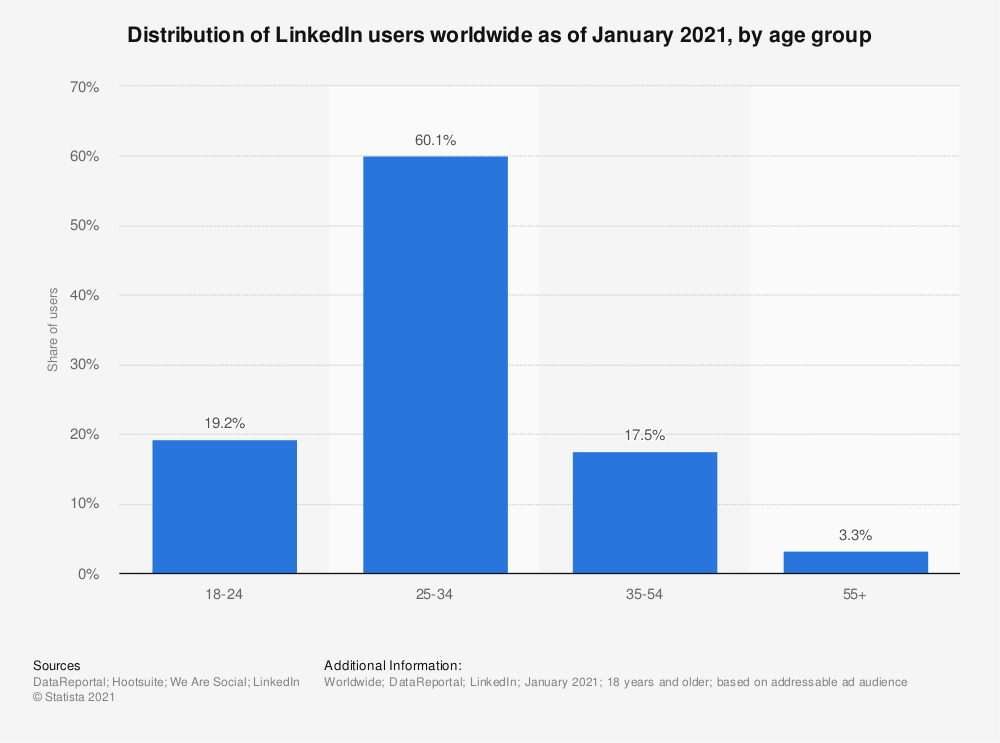
\includegraphics[height=10cm]{Figures/linkedin users.png}
	\caption{Distribution of LinkedIn users worldwide as of January 2021, by age group}
	\label{fig:linkedin_users}
\end{figure}


\subsection{Sample Interview Questions}
\begin{enumerate}
	\item What are the common scenarios that you are using LinkedIn search function?
	\item What group of people you are using LinkedIn search function to search for?
\end{enumerate}

\subsection{Sample Survey Questions}
\begin{enumerate}
	\item On a scale 1 - 5, 1 being the easiest, how easy to find your co-workers by name on LinkedIn My Network page?
	\item On a scale 1 - 5, 1 being the easiest, how easy to find conference speakers by name on LinkedIn mobile app?
\end{enumerate}

\end{document}